\documentclass[a4paper, 12pt]{article}

\usepackage[utf8]{inputenc}
\usepackage[T1]{fontenc}
\usepackage{textcomp}
\usepackage{listings}
\usepackage{lmodern}
\usepackage{amsfonts}
\usepackage{titling}
\usepackage{lipsum}
\usepackage[left=1in, right=1in, bottom=1in, top=1in]{geometry}
\usepackage{amsthm}
\usepackage{tcolorbox}
\usepackage{hyperref}
\usepackage{xcolor}
\usepackage{graphicx}
\usepackage{makeidx}
\usepackage{tikz}
\usepackage{svg}
\usepackage{cases}
\usepackage{apacite}
\usepackage{tkz-berge}
\usepackage{url}
\usepackage{tgtermes}
\usepackage{sectsty}
\usepackage{subcaption}
\usepackage{setspace}
\usepackage{float}
\usepackage{amsmath, amssymb}


% figure support
\definecolor{tugblue}{HTML}{33588B}
\allsectionsfont{\color{tugblue}}
\newcommand{\coloredrule}[2][tugblue]{%
  \textcolor{#1}{\rule{\linewidth}{#2}}%
}

\usepackage{import}
\usepackage{xifthen}
\pdfminorversion=7
\usepackage{pdfpages}
\usepackage{transparent}
\usepackage{color}
\newcommand{\incfig}[2][1]{%
    \def\svgwidth{#1\columnwidth}
    \import{./figures/}{#2.pdf_tex}
}

%mathstyling
\theoremstyle{plain}
\newtheorem{thm}{Theorem}[section]
\newtheorem{lem}[thm]{Lemma}
\newtheorem{prop}[thm]{Proposition}
\newtheorem*{cor}{Corollary}

\theoremstyle{definition}
\newtheorem{defn}{Definition}[section]
\newtheorem{conj}{Conjecture}[section]
\newtheorem{exmp}{Example}[section]
\newtheorem{axiom}{Axiom}
\theoremstyle{remark}
\newtheorem*{rem}{Remark}
\newtheorem*{note}{Note}

\definecolor{darkgreen}{rgb}{0.0, 0.5, 0.0}

\pdfsuppresswarningpagegroup=1
\lstset{
tabsize = 4, %% set tab space width
showstringspaces = false, %% prevent space marking in strings, string is defined as the text that is generally printed directly to the console
numbers = left, %% display line numbers on the left
commentstyle = \color{darkgreen}, %% set comment color
keywordstyle = \color{blue}, %% set keyword color
stringstyle = \color{red}, %% set string color
rulecolor = \color{black}, %% set frame color to avoid being affected by text color
basicstyle = \small \ttfamily , %% set listing font and size
breaklines = true, %% enable line breaking
numberstyle = \tiny,
  frame=none,
  xleftmargin=2pt,
  stepnumber=1,
  belowcaptionskip=\bigskipamount,
  captionpos=b,
  escapeinside={*'}{'*},
  language=haskell,
  tabsize=2,
  emphstyle={\bf},
  showspaces=false,
  columns=flexible,
  showstringspaces=false,
  morecomment=[l]\%,
}
\begin{document}
	\begin{titlepage}
	        \vspace*{0.8cm}
	        \begin{center}
	                \coloredrule{2pt}\par
	                \vskip 0.6cm
	                \textbf{\Huge Knowledge Discovery in Databases}\par
	                \vskip 0.3cm
	                \coloredrule{2pt}\par
	
	                \vskip 3cm
	
	                \includesvg[width=0.4\textwidth]{gabrovo}
	
	                \vspace{3cm} % small space before your name and info
	                \Large CEM YILMAZ \\
	                \Large Technical University of Gabrovo \\
	                \Large Faculty of \\
	                \Large\textit{Electrical Engineering and Electronics}\\
	
	                \vspace{2cm}
	                \Large Notes made for the degree of\\
	                \Large \textit{Software and Computer Engineering}\\
	                \Large \today \\
	                \vspace{0.5cm}
	
	                \vfill  % Pushes content up from bottom
	        \end{center}
	\end{titlepage}
	
	\tableofcontents
	\newpage
	\section{Introduction}
	\subsection{Artificial Intelligence (AI)}
\noindent This module focuses on the techniques used to extract data from data. In particular, we cover statistical methods, the use of data, and techniques to extract useful information. Data mining is especially useful for artificial intelligence (AI), which is a field that encompasses development of intelligent machines, systems and algorithms that exhibit human-like intelligence. The goal is to provide the ability of machines to perceive, reason, learn and make decisions based on data.

\begin{tcolorbox}[colback=black!3!white,colframe=black!60!white,title=\begin{defn}Artificial Intelligence (AI) \label{Artificial Intelligence (AI)}\end{defn}]
A field that encompasses the development of intelligent machine systems that exhibit human-like intelligence. The goal is to provide the ability of machines to perceive, reason, learn and make decisions based on data.
\end{tcolorbox}
\noindent The AI as a field has multiple different methods of creating AI.
\begin{figure}[H]
	\centering
	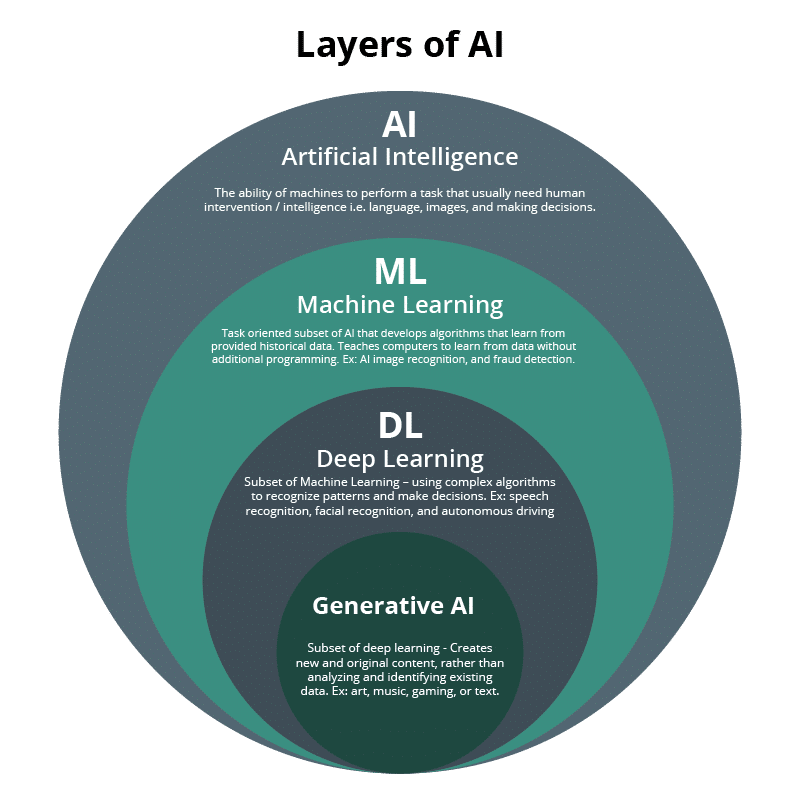
\includegraphics[width=0.8\textwidth]{figures/layers_of_ai.png}
	\caption{Layers of AI}
	\label{fig:figures-layers_of_ai-png}
\end{figure}
\noindent It follows that
\begin{align*}
	\text{Generative AI} \subset \text{Deep Learning} \subset \text{Machine Learning} \subset \text{Artificial Intelligence}
\end{align*}
\begin{itemize}
	\item \textbf{Artificial Intelligence}: the superset of AI and encompasses all techniques known. However, for techniques that belong in the AI set and not the ML set include old techniques such as rule-based AIs, constraint satisfaction problem solving AI algorithms, heuristic algorithms e.g. A* search, minimax, etc. Such AIs are called symbolic AIs. 
	\item \textbf{Machine Learning}: the subset of AI, contains statistical methods to infer about existing data and create predictions using such data. Examples include the kernel trick, support vector machines (SVMs), principle components analysis (PCA), dimensionality reduction, etc. Learning can be done through supervised, unsupervised, or reinforced.
	\item \textbf{Deep Learning}: subset of Machine Learning, deep learning uses artificial neural networks like perceptrons, with multiple layers to learn hierarchal representation of a given data. This method generally requires training and learning methods using techniques such as optimisers and back-propogation. This type of AI is especially good in image classification (CNNs), pattern recognition and language processing (RNNs) (Transformers). Unfortunately, it is hard to learn the way deep learning neural networks work, and are generally interpreted as black boxes.
	\item \textbf{Evolutionary Computation}: These algorithms and class of AIs use genetic algorithms e.g. inheritance, mutations in their code and set of rules. It is a specific part of niche AI.
\end{itemize}
The difference between ML and DL is that a human designs and selects features a model should use in its task. A deep learning architecture instead learns features directly from data. Indeed, the applications of AI can be seen everywhere today: medical healthcare e.g. analysis of images, data; finance for the analysis of fraud detection, credit scoring, stock exchange; social media e.g. analysis of psychological profile using unsupervised clustering; transportation and logistics e.g. help optimise routes, weights, manage supply chains; and more.
\subsection{Data Mining}
Data mining is not to be confused with artificial intelligence. Data mining is the process extracting and discovering patterns in large data sets. The primary goal is to identify patterns or trends that may not be immediately obvious or detectable by humans. Data mining techniques are used in AI to extract knowledge from data sets. Several data mining techniques exist to extract information from a data set:
\begin{itemize}
	\item \textbf{Classification}: separate labels (classes) from large datasets
	\item Clustering: idea of putting labels onto data points that are similar to each other, i.e. creating groups
	\item \textbf{Regression analysis}: predicting continuous numerical values based on input variables.
	\item \textbf{Evolutionary optimisation algorithms}: ant colony optimisation, swarm optimisation, genetic programming, mimicking the process of natural selection.
	\item \textbf{Hybrid approaches}: combines multiple methods together.
\end{itemize}
\subsection{Questions}
\begin{enumerate}
	\item What is the main purpose of artificial intelligence and what are some of its main applications?
	\item What is machine learning and what are some of the ways in which it differs from deep machine learning?
	\item How does AI relate to data mining and how can it improve the data mining process?
	\item What are the main data mining techniques and how do they contribute to data processing and large volumes of data?
	\item What are the main differences between artificial intelligence and data mining, and how do they together improve information processing and analysis?
\end{enumerate}
\subsection{Answers}
\begin{enumerate}
	\item Artificial intelligence is a field consisting of systems and algorithms used to perform tasks involving reasoning, interpretation, learning and application of data similar to what a human would do. Some of the main applications include in healthcare e.g. image analysis for cancer tumours; finance e.g. credit score analysis, risk analysis; logistics e.g. optimising routes from point A to B based on multiple constraints, and more.
	\item Machine learning is a subfield of artificial intelligence that utilises statistical methods such as linear regression, support vector machine, kernels etc. to discover and find patterns in data, and create predictions for data. In machine learning, it is the human that selects which features are to be analysed, and how. In deep learning, these features are not selected, but are rather learned by the system, meaning the human does not select features to be analysed, however, the human can still choose how deep it should learn features. In traditional machine learning, humans often design or select the features to be analysed. Deep learning uses neural networks with multiple layers to learn feature representations automatically from data. However, humans still choose the input data, network architecture, number of layers and neurons, and training settings such as the optimiser. 
	\item Data mining is the process of extracting useful data using statistical and AI methods, and these findings can additionally be fed back into AI for support. In particular, since AI is a field that includes algorithms and systems that utilise data to solve problems that would require a human to use reason and logic, data mining would be the process that the AI extracts information from. AI can improve the data mining process through known algorithms that also do data mining. For example, clustered unsupervised learning could group data together and give you an output. Additionally, AI can learn what data is good through reinforcement learning, create predictions for future data, and even extract features on its own using neurons and layers, although this creates a "black box", which is hard to analyse on which features and how they were extracted.
	\item Clustering is a method of grouping data under the same label, which be based on distance in a graph, or other features such as values. Classification is the idea of labelling every data point based on where they belong e.g. this is a dog, this is a cat, or a bird. Regression analysis is the analysis of data points based on coordinate system using variables, can also be multi dimensional. It helps you predict next points, find error of your analysis for accuracy, where you can interpolate or extrapolate. You can also use hybrid approaches, where you combine different data processing techniques. For example, you can combine k-means to classify new points without using AI, but first establish clustering based on unsupervised deep learning model.
	\item Two points: AI can be used as a data mining tool, for example clustering. Additionally, data mining output can also be used to train AI and improve AI using patterns and information it has discovered. For example, you can use linear regression analysis between two variables to predict another point's values. The main difference between the both is the following: data mining is the process of extracting and finding useful patterns in a data set. Artificial intelligence, on the other hand, is a field with algorithms and systems which imitate human reasoning through learning, reasoning and decision-making to solve complex problems.
\end{enumerate}
\newpage
\section{Data Mining}
\subsection{What is Data Mining?}
\begin{tcolorbox}[colback=black!3!white,colframe=black!60!white,title=\begin{defn}Data Mining \label{Data Mining}\end{defn}]
The process of extracting knowledge from huge datasets by using statistical and computational algorithms, machine learning approaches and pattern recognition techniques. The goal is to discover hidden patterns, trends and associations that can be used for decision-making.
\end{tcolorbox}
\noindent Data extraction and the process of data mining involves several steps:
\begin{enumerate}
	\item \textbf{Data collection}: the first step is to gather relevant data from various sources. This may include gaining access to databases, extracting information from the WWW, extracting data from documents or other sources.
	\item \textbf{Data cleaning}: the second step is to clean the data to ensure analysis can be made. This includes making sure type data for data is relevant, null entries are dropped or filled in, removing irrelevant information, get rid of low quality rows, etc., outliers dropped, etc.
	\item \textbf{Data integration}: data can be scattered across multiple sources or stored in different formats, and they must be combined into a single comprehensive data set which can facilitate analysis.
	\item Data transformation: Data may need to be transformed or restructured to facilitate the extraction process. This may include specific numerical representations, normalisation and other transformations that may be required depending on the algorithms used for analysis.
	\item \textbf{Knowledge interpretation}: The final step is to interpret the discovered knowledge which can be used to make decisions, improve existing processes and gain a deeper understanding of the underlying problem.
\end{enumerate}
Additionally, the data mining techniques can be categorised as:
\begin{enumerate}
	\item \textbf{Classification}: assigning classes or categories based on their characteristics which can be used to predict unseen data into which category it belongs.
	\item \textbf{Clustering}: clustering categorises groups based on their inherent properties. It does not require prior class definition and can automatically identify hidden structures in the data.
	\item Association rule extraction: discovers relationships or associations between items in large datasets. 
	\item \textbf{Anomaly detection}: used to find rare or unusual instances or patterns that deviate from the norm, i.e. finding outliers. 
	\item \textbf{Text mining}: extracting useful information and patterns from unstructured text data such as documents, emails, social media posts, customer reviews, etc.
	\item \textbf{Time series analysis}: analyse data collected over time to identify patterns and trends. Especially used for financial forecasting.
\end{enumerate}
Data mining is used in finance and banking, healthcare, business and marketing, social media and web analytics, etc.
\subsection{History of Data Mining}
Data mining started becoming popular in approximately 1980s and 1990s. In 1996, Usama Fayyad, Gregory Piatetsky-Shapiro and Padhraic Smyth introduce the Database Knowledge Discovery Process Model that provides a systematic framework for knowledge discovery and today has become the standard model. Since the framework, important advances have been made in the tools used for data mining, in particular:
\begin{itemize}
	\item \textbf{Decision Trees}: new algorithms such as ID3, C4.5
	\item \textbf{Neural Networks}: inspired by the functioning of the human brain, using interconnected nodes.
	\item \textbf{Support Vector Machines (SVMs)}: particularly effective for classification and regression tasks and has found applications in area such as image recognition, text categorisation and bioinformatics.
	\item \textbf{Clustering algorithms}: k-means, hierarchical clustering, density-based clustering.
	\item \textbf{Association rule extraction}: the techniques used for association rules such as Apriori algorithms.
\end{itemize}
The timeline of data mining is as follows:
\begin{itemize}
	\item \textbf{1960}: birth of the data mining concept, researchers explore techniques for extracting knowledge.
	\item \textbf{1970}: researchers delve deeper into the field of statistical modeling and developing methodologies for analysing data.
	\item \textbf{1990}: the term "data mining" is defined to describe the process of extracting valuable information from large data sets. Organisations are realising the potential to gain competitive advantage and start making informed decisions.
	\item \textbf{2000}: emergence of big data with rapid growth of digital information increases the importance and scope of data mining.
	\item \textbf{2010}: ethical issues and privacy concerned related to data mining become realised. Organisations now focus on responsible data mining, practices, and protecting sensitive information.
	\item \textbf{2020}: integrating data mining with artificial intelligence, specifically machine learning to accelerate data mining capabilities. Advanced techniques such as deep learning and reinforcement learning increase accuracy and enable more complex analyses.
\end{itemize}
\subsection{Application of Data Mining}
\begin{itemize}
	\item \textbf{Retail and e-commerce}: understanding customer behaviour and preferences is essential for success e.g. analysing browsing history, patterns, demographics, personalise campaigns, optimise pricing strategies and improve inventory management.
	\item \textbf{Healthcare and medical research}: improving patient care, disease management, medical research, electronic health records, medical imaging data, genetic information can all be used to identify patterns and predict disease outcomes and even recommend treatment.
	\item \textbf{Financial services}: fraud detection, risk assessment, customer relationship management by analysing transactions.
	\item \textbf{Manufacturing and supply chain management}: optimise production processes, improve quality control, reduce costs by analysing sensor data and historical product data.
	\item \textbf{Telecommunications}: customer segmentation, churn prediction, network optimisation by analysing detailed call records, customer demographics, usage patterns, network traffic data.
	\item \textbf{Social media and sentiment analysis}: data including text, images, videos, can be analysed and used to extract valuable information about customer opinions, preferences and trends to improve customer satisfaction.
	\item \textbf{Transport and logistics}: used in aiding efficient route planning, demand forecasting, fleet optimisation. It is used to predict demand fluctuations, allowing companies to optimise their routes, allocate resources more efficiently, and reduce transportation costs.
	\item \textbf{Energy}: data mining helps optimise energy consumption, predictive maintenance, smart grid management, optimise energy distribution by analysing consumption patterns. 
\end{itemize}
\subsection{Questions}
\begin{enumerate}
	\item What is data mining and why is it important in the modern information world?
	\item What is the historical path development of data mining techniques, what are the contemporary challenges and future directions?
	\item What are the main areas in which data mining is applied, and how can this process contribute to optimising and improving activities in these areas?
	\item What are some of the applications of data mining healthcare and medical research? How do these apps improve the healthcare sector?
	\item Explain how data mining is used in the financial services field and what advantages this process can bring to the financial industry.
	\item How do social media and sentiment analysis relate to data mining? What information can be extracted from social media and how can it be used?
\end{enumerate}
\subsection{Answers}
\begin{enumerate}
	\item Data mining is the process of extracting, cleaning, analysing, and interpreting a dataset. It is important because in today's age, data is found abundantly using the internet and all competitors, businesses etc. use it to optimise their production, advertisements and market presence, giving them an edge over competitors that do not.
\end{enumerate}
\newpage
\section{Data Preprocessing}
\subsection{Data Cleaning}
Also known as data scrubbing, involves identifying and correcting errors, inconsistencies and inaccuracies in datasets to ensure quality and reliability. It is essential for the following reasons:
\begin{itemize}
	\item \textbf{Accurate analysis}: accurate analysis requires accurate and reliable data. If it is corrupt or inaccurate, you may obtain erroneous analyses, interpretations, patterns and conclusions.
	\item \textbf{Consistency}: inconsistent data formats such as dates, numbers, naming conventions can hinder data integration and data analysis.
	\item \textbf{Outlier detection}: data points that deviate significantly from the rest of the data set (outliers) can distort obtained results from analyses. Data cleaning involves detecting and eliminating such deviations.
	\item \textbf{Improved data quality}: Data cleaning techniques such as deduplication, recording rules and constraints for accurate and reliable results.
\end{itemize}
There are many ways to handle missing values, including deletion or imputation (estimating values). For duplicate entries, you can delete them. Fixing inconsistent formatting will require to standardise the field. For deviations, you can winsorise it (replaced with the nearest values within a specific percentile range) or delete it. Integration of inconsistent data can be done using data harmonisation and linking records. 
\end{document}
